
This section performs ablation studies on the validation set of five datasets that share horizon lengths, \ETTm$_2$, \Exchange, \Electricity, \TrafficL, and \Weather. The section's experiments control for \ours\ settings described in Table~\ref{table:hyperparameters}, only varying a single characteristic of interest of the network and measuring the effects in validation.

% -------------------------------------------------------------------------------------------------------------
% \clearpage
\subsubsection{Pooling Configurations}
\label{appendix:ablation_pooling_configurations}
% -------------------------------------------------------------------------------------------------------------

\begin{figure}[ht!]
\centering
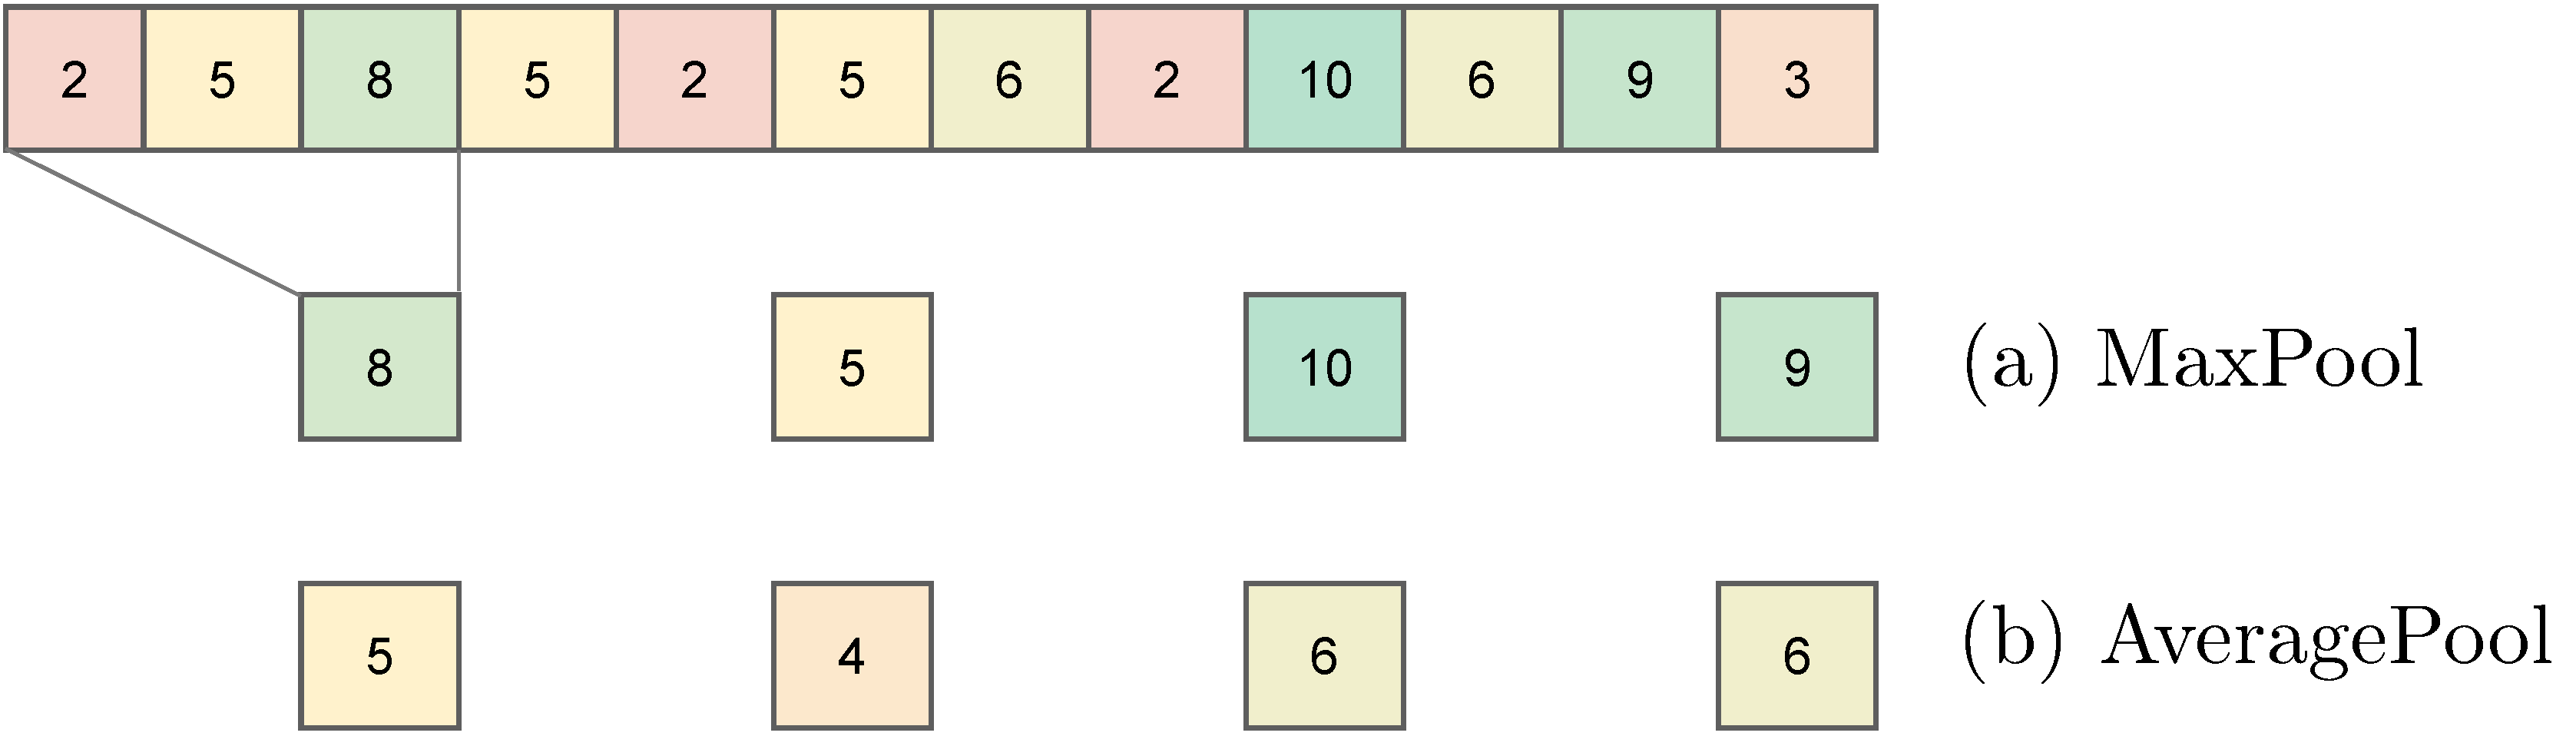
\includegraphics[width=0.7\linewidth]{images/Pooling.pdf}
\caption{Proposed pooling configurations.} \label{fig:pooling_appendix}
\end{figure}


In Section~\ref{section:multirate_sampling} we described the \emph{multi-rate signal sampling} enhancement of the \ours\ architecture. Here we conduct a study to compare the accuracy effects of different pooling alternatives, on Equation~(\ref{equation:nhits_mixed_datasampling}). We consider the MaxPool and AveragePool configurations.

As shown in Table~\ref{table:ablation_pooling}, the MaxPool operation consistently outperforms the AveragePool alternative, with MAE improvements up to 15\% and MSE up to 8\% in the most extended horizon. On average, the forecasting accuracy favors the MaxPool method across the datasets and horizons. 
%We conducted the main experiments of this work with this technique.

\begin{table}[!ht] %ht!
% \footnotesize
%\tiny
\scriptsize
    \begin{center}
    \caption{Empirical evaluation of long multi-horizon multivariate forecasts for \ours\ with different pooling configurations. All other hyperparameters were kept constant across all datasets. MAE and MSE for predictions averaged over eight seeds, the best result is highlighted in bold (lower is better). Average percentage difference relative to average pooling in the last panel.}
    \label{table:ablation_pooling}
	\begin{tabular}{ll | cccccc} \toprule
    						        &     & \multicolumn{2}{c}{MaxPool}  & \multicolumn{2}{c}{AveragePool}        \\
    						        &     & MSE             & MAE             & MSE            & MAE              \\ \midrule
\parbox[t]{1mm}{\multirow{4}{*}{\rotatebox[origin=c]{90}{\ETTm$_{2}$}}}
									& 96  & \textbf{0.185}  & 0.265           & 0.186          & \textbf{0.262}   \\
									& 192 & \textbf{0.244}  & \textbf{0.308}  & 0.257          & 0.315            \\
									& 336 & \textbf{0.301}  & \textbf{0.347}  & 0.312          & 0.356            \\
									& 720 & \textbf{0.429}  & \textbf{0.438}  & 0.436          & 0.447            \\ \midrule
\parbox[t]{1mm}{\multirow{4}{*}{\rotatebox[origin=c]{90}{\Electricity}}}
									& 96  & \textbf{0.152}  & \textbf{0.257}  & 0.181          & 0.290            \\
									& 192 & \textbf{0.172}  & \textbf{0.275}  & 0.212          & 0.320            \\
									& 336 & \textbf{0.197}  & \textbf{0.304}  & 0.238          & 0.343            \\
									& 720 & \textbf{0.248}  & \textbf{0.347}  & 0.309          & 0.400            \\ \midrule
\parbox[t]{1mm}{\multirow{4}{*}{\rotatebox[origin=c]{90}{\Exchange}}}
									& 96  & \textbf{0.109}  & \textbf{0.232}  & 0.112          & 0.238            \\
									& 192 & 0.280           & 0.375           & \textbf{0.265} & \textbf{0.371}   \\
									& 336 & \textbf{0.472}  & 0.504           & 0.501          & \textbf{0.502}   \\
									& 720 & \textbf{1.241}  & \textbf{0.823}  & 1.610          & 0.942            \\ \midrule
\parbox[t]{1mm}{\multirow{4}{*}{\rotatebox[origin=c]{90}{\TrafficL}}}
									& 96  & \textbf{0.405}  & \textbf{0.286}  & 0.468          & 0.332            \\
									& 192 & \textbf{0.421}  & \textbf{0.297}  & 0.490          & 0.347            \\
									& 336 & \textbf{0.448}  & \textbf{0.318}  & 0.531          & 0.371            \\
									& 720 & \textbf{0.527}  & \textbf{0.362}  & 0.602          & 0.400            \\ \midrule
\parbox[t]{1mm}{\multirow{4}{*}{\rotatebox[origin=c]{90}{\Weather}}}
									& 96  & \textbf{0.164}  & \textbf{0.199}  & 0.167          & 0.200            \\
									& 192 & \textbf{0.224}  & \textbf{0.255}  & 0.226          & 0.255            \\
									& 336 & 0.285           & 0.311           & \textbf{0.284} & \textbf{0.297}   \\
									& 720 & 0.366           & 0.359           & \textbf{0.360} & \textbf{0.352}   \\ \midrule \midrule
\parbox[t]{1mm}{\multirow{4}{*}{\rotatebox[origin=c]{90}{P. Diff.}}}
									& 96  & \textbf{-8.911} & \textbf{-6.251} & 0.000          & 0.000            \\
									& 192 & \textbf{-7.544} & \textbf{-6.085} & 0.000          & 0.000            \\
									& 336 & \textbf{-8.740} & \textbf{-4.575} & 0.000          & 0.000            \\
									& 720 & \textbf{-15.22} & \textbf{-8.318} & 0.000          & 0.000            \\ \bottomrule
	\end{tabular}
	\end{center}
\end{table}

% -------------------------------------------------------------------------------------------------------------
%\clearpage
% \vspace{14mm}
\subsubsection{Interpolation Configurations}
\label{appendix:ablation_interpolation_configurations}
% -------------------------------------------------------------------------------------------------------------

\begin{figure}[!ht]
\centering
\subfigure[N.Neighbor]{\label{fig:interpolation_nn}
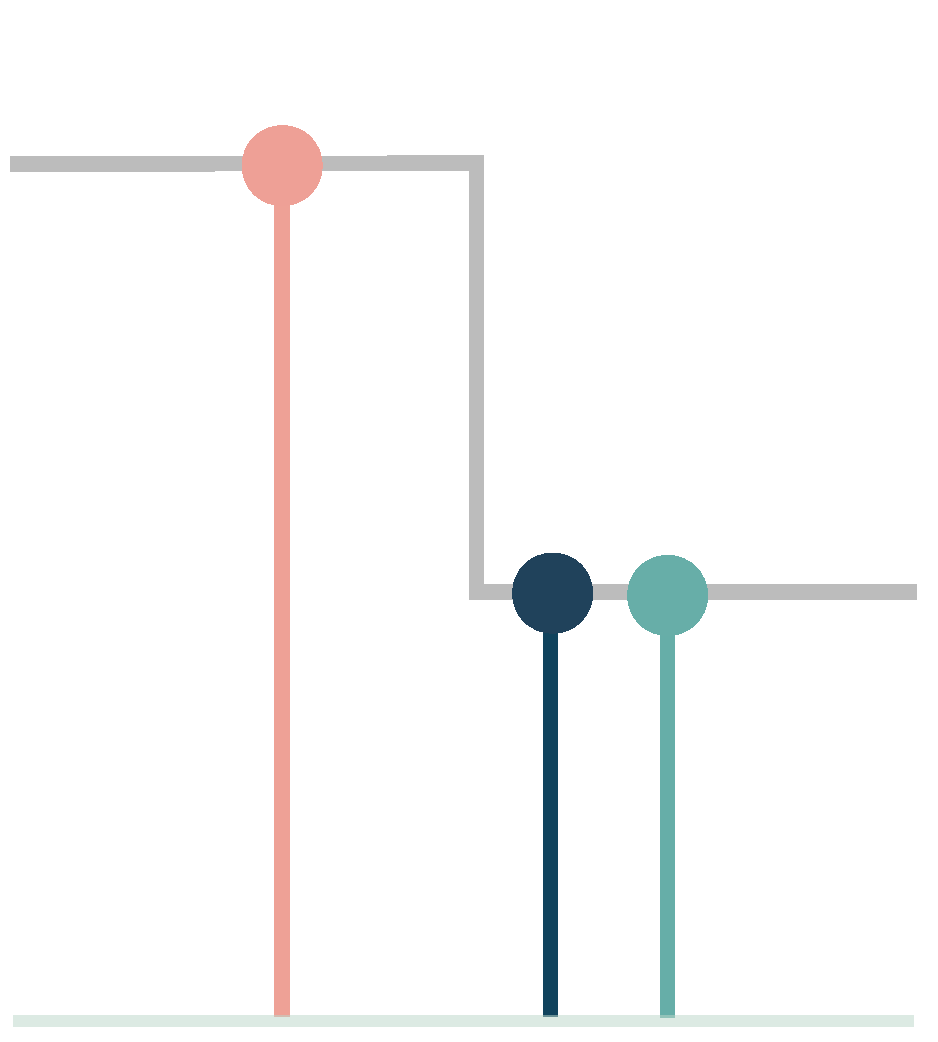
\includegraphics[width=0.15\linewidth]{images/Interpolation2.pdf}} %0.23
\subfigure[Linear]{\label{fig:interpolation_linear}
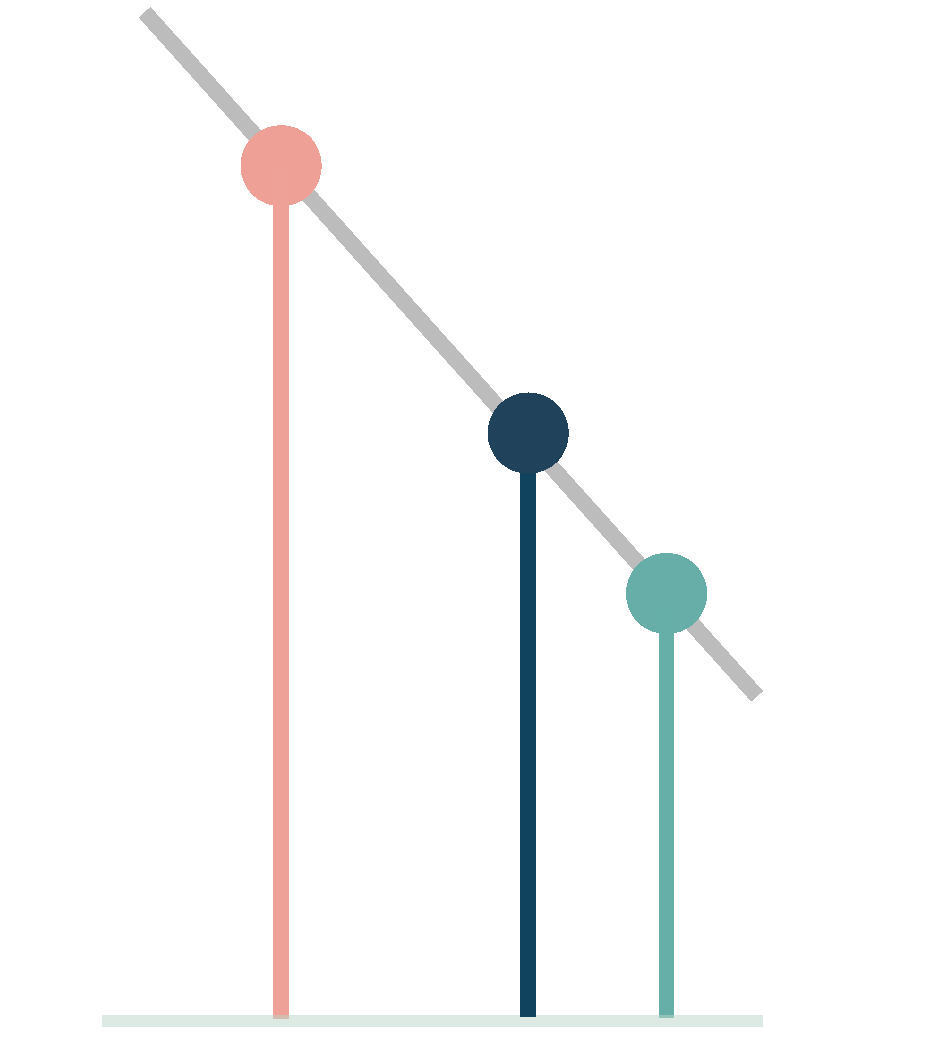
\includegraphics[width=0.15\linewidth]{images/Interpolation1.pdf}} %0.23
\subfigure[Cubic]{\label{fig:interpolation_cubic}
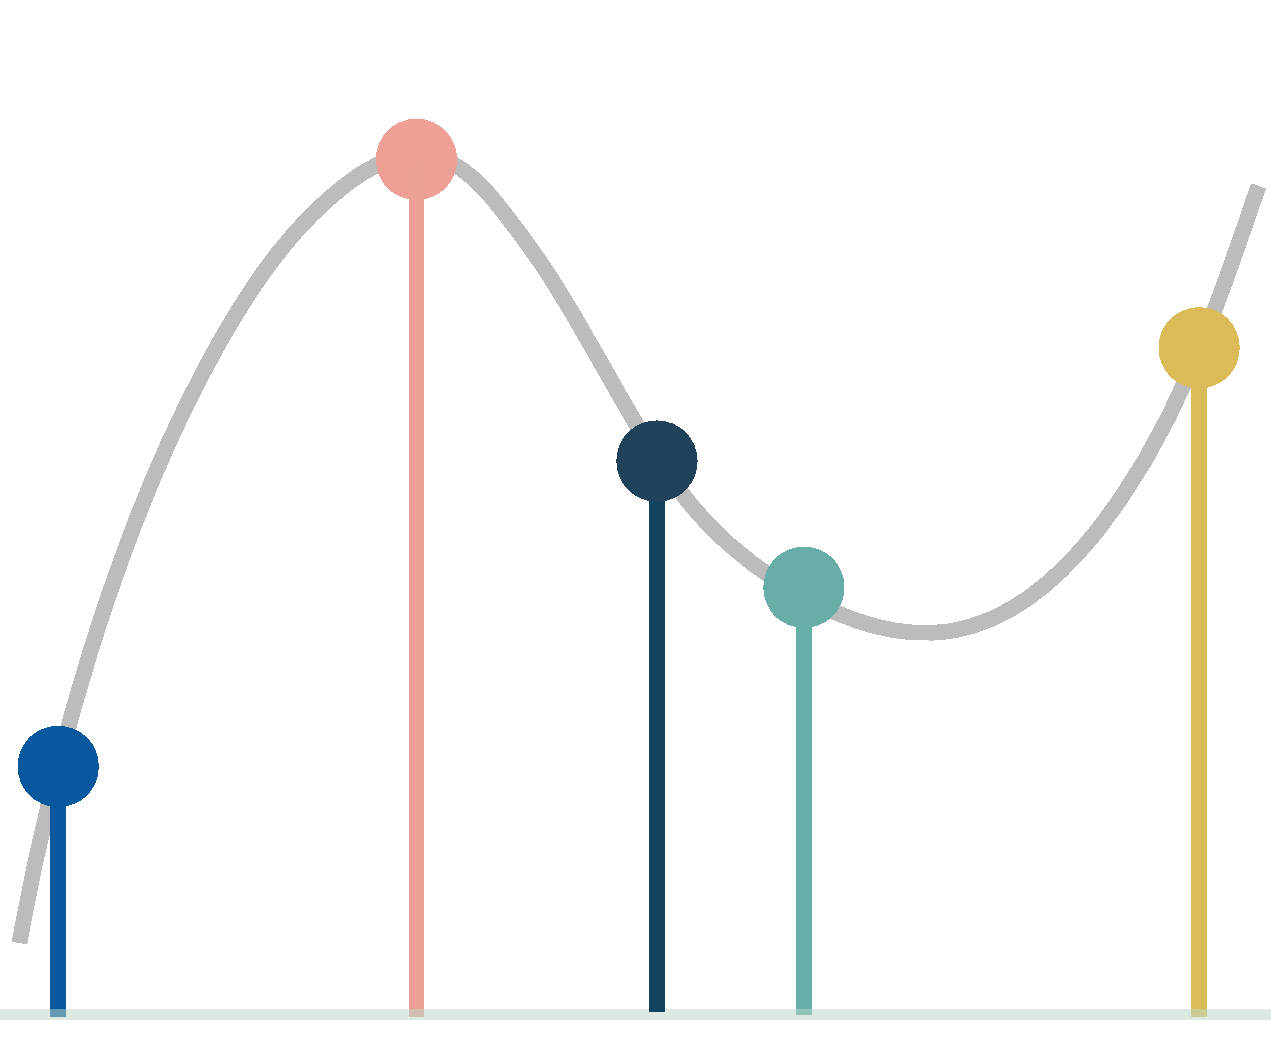
\includegraphics[width=0.22\linewidth]{images/Interpolation3.pdf}} %0.3
\caption{Proposed interpolator configurations.} \label{fig:interpolation_appendix}
\end{figure}

In Section~\ref{section:hierarchical_interpolation} we described the \emph{hierarchical interpolation} enhancement of the multi-step prediction strategy. Here we conduct a study to compare the accuracy effects of different interpolation alternatives. To do it, we change the interpolation technique used in the multi-step forecasting strategy of the \ours\ architecture. The interpolation techniques considered are nearest neighbor, linear and cubic. We describe them in detail below.

Recalling the notation from Section~\ref{section:hierarchical_interpolation}, consider the time indexes of a multi-step prediction $\tau \in \{t+1,\dots,t+H\}$, let $\mathcal{T}=\{t+1,t+1+1/r_{\ell}\dots,t+H\}$ be the anchored indexes in \ours\ layer $\ell$, and the forecast $\hat{y}_{\tau,\ell} = g(\tau, \btheta^{f}_{\ell})$ and backast $\tilde{y}_{\tau,\ell} = g(\tau, \btheta^{f}_{\ell})$ components. Here we define different alternatives for the interpolating function $g \in \mathcal{C}^{0}, \mathcal{C}^{1}, \mathcal{C}^{2}$. For simplicity we skip the $\ell$ layer index.

\textbf{Nearest Neighbor.} In the simplest interpolation, we use the anchor observations in the time dimension closest to the observation we want to predict. Specifically, the prediction is defined as follows:
\begin{equation}
    \hat{y}_{\tau}
    = \theta[t^{*}]  \quad \text{with} \quad t^{*} = \text{argmin}_{t\in \mathcal{T}}\{|t-\tau|\}
    \label{equation:interpolation_nearest}
\end{equation}

\textbf{Linear.} An efficient alternative is the linear interpolation method, which uses the two closest neighbor indexes $t_{1}$ and $t_{1}$, and fits a linear function that passes through both.
\begin{equation}
    \hat{y}_{\tau}
    = \left(\theta[t_{1}] + \left(\frac{\theta[t_{2}]-\theta[t_{1}]}{t_{2}-t_{1}}\right)(\tau-t_{1})\right)
    \label{equation:interpolation_linear2}
\end{equation}

\textbf{Cubic.} Finally we consider the Hermite cubic polynomials defined by the interpolation constraints for two anchor observations $\theta_{t_{1}}$ and $\theta_{t_{1}}$ and its first derivatives $\theta^{'}_{t_{1}}$ and $\theta^{'}_{t_{1}}$.
\begin{equation}
    \hat{y}_{\tau}
    = \theta[t_{1}] \phi_{1}(\tau) + \theta[t_{2}] \phi_{2}(\tau) +
      \theta^{'}[t_{1}] \psi_{1}(\tau) + \theta^{'}[t_{2}]\psi_{2}(\tau)
    \label{equation:interpolation_cubic}
\end{equation}

With the Hermite cubic basis defined by:
\begin{subequations}
\begin{alignat}{3} 
    \phi_{1}(\tau) = 2 \tau^{3}-3\tau^{2} + 1 \\
    \phi_{2}(\tau) = -2 \tau^{3}+ 3\tau^{2} \\
    \psi_{1}(\tau) = \tau^{3}-2\tau^{2} + \tau \\
    \psi_{2}(\tau) = \tau^{3}-\tau^{2}
\end{alignat}
\end{subequations}

The ablation study results for the different interpolation techniques are summarized in Table~\ref{table:ablation_interpolation}, we report the average MAE and MSE performance across the five datasets. Figure ~\ref{fig:decomposition_pooling} presents the decomposition for the different interpolation techniques. We found that linear and cubic interpolation consistently outperform the nearest neighbor alternative, and show monotonic improvements relative to the nearest neighbor technique along the forecasting horizon. 

% \clearpage
\begin{figure*}[ht!]
\centering
\subfigure[Nearest neighbor interpolation]{\label{fig:decomposition_nearest}
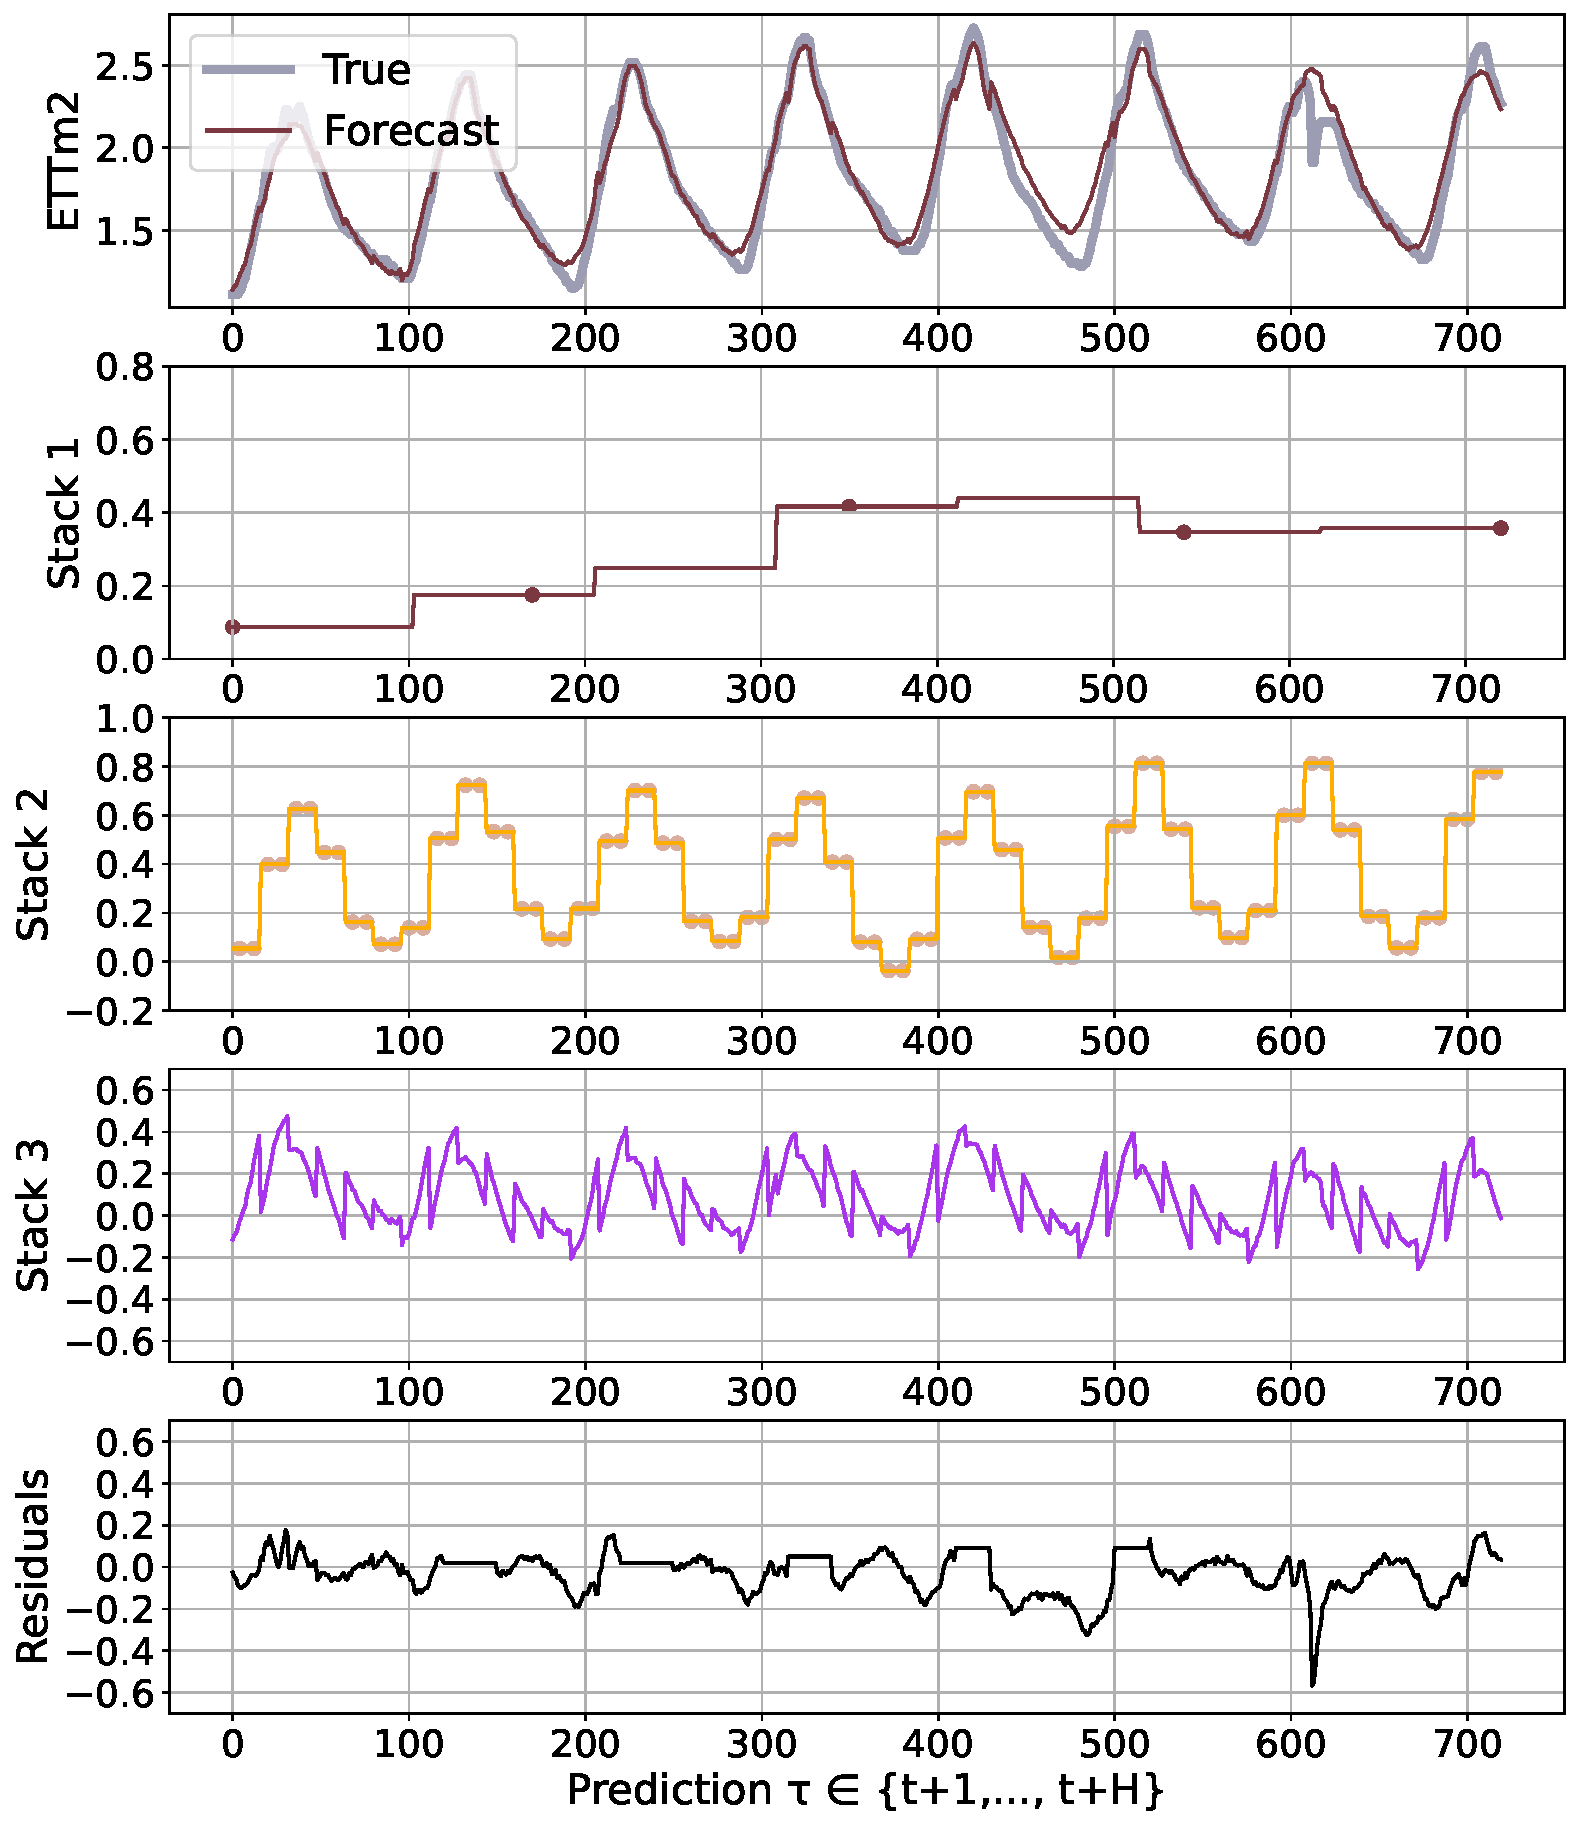
\includegraphics[width=0.48\linewidth]{images/plots-interpetable-decomposition-nearest.pdf}}
\subfigure[Linear interpolation]{\label{fig:decomposition_linear2}
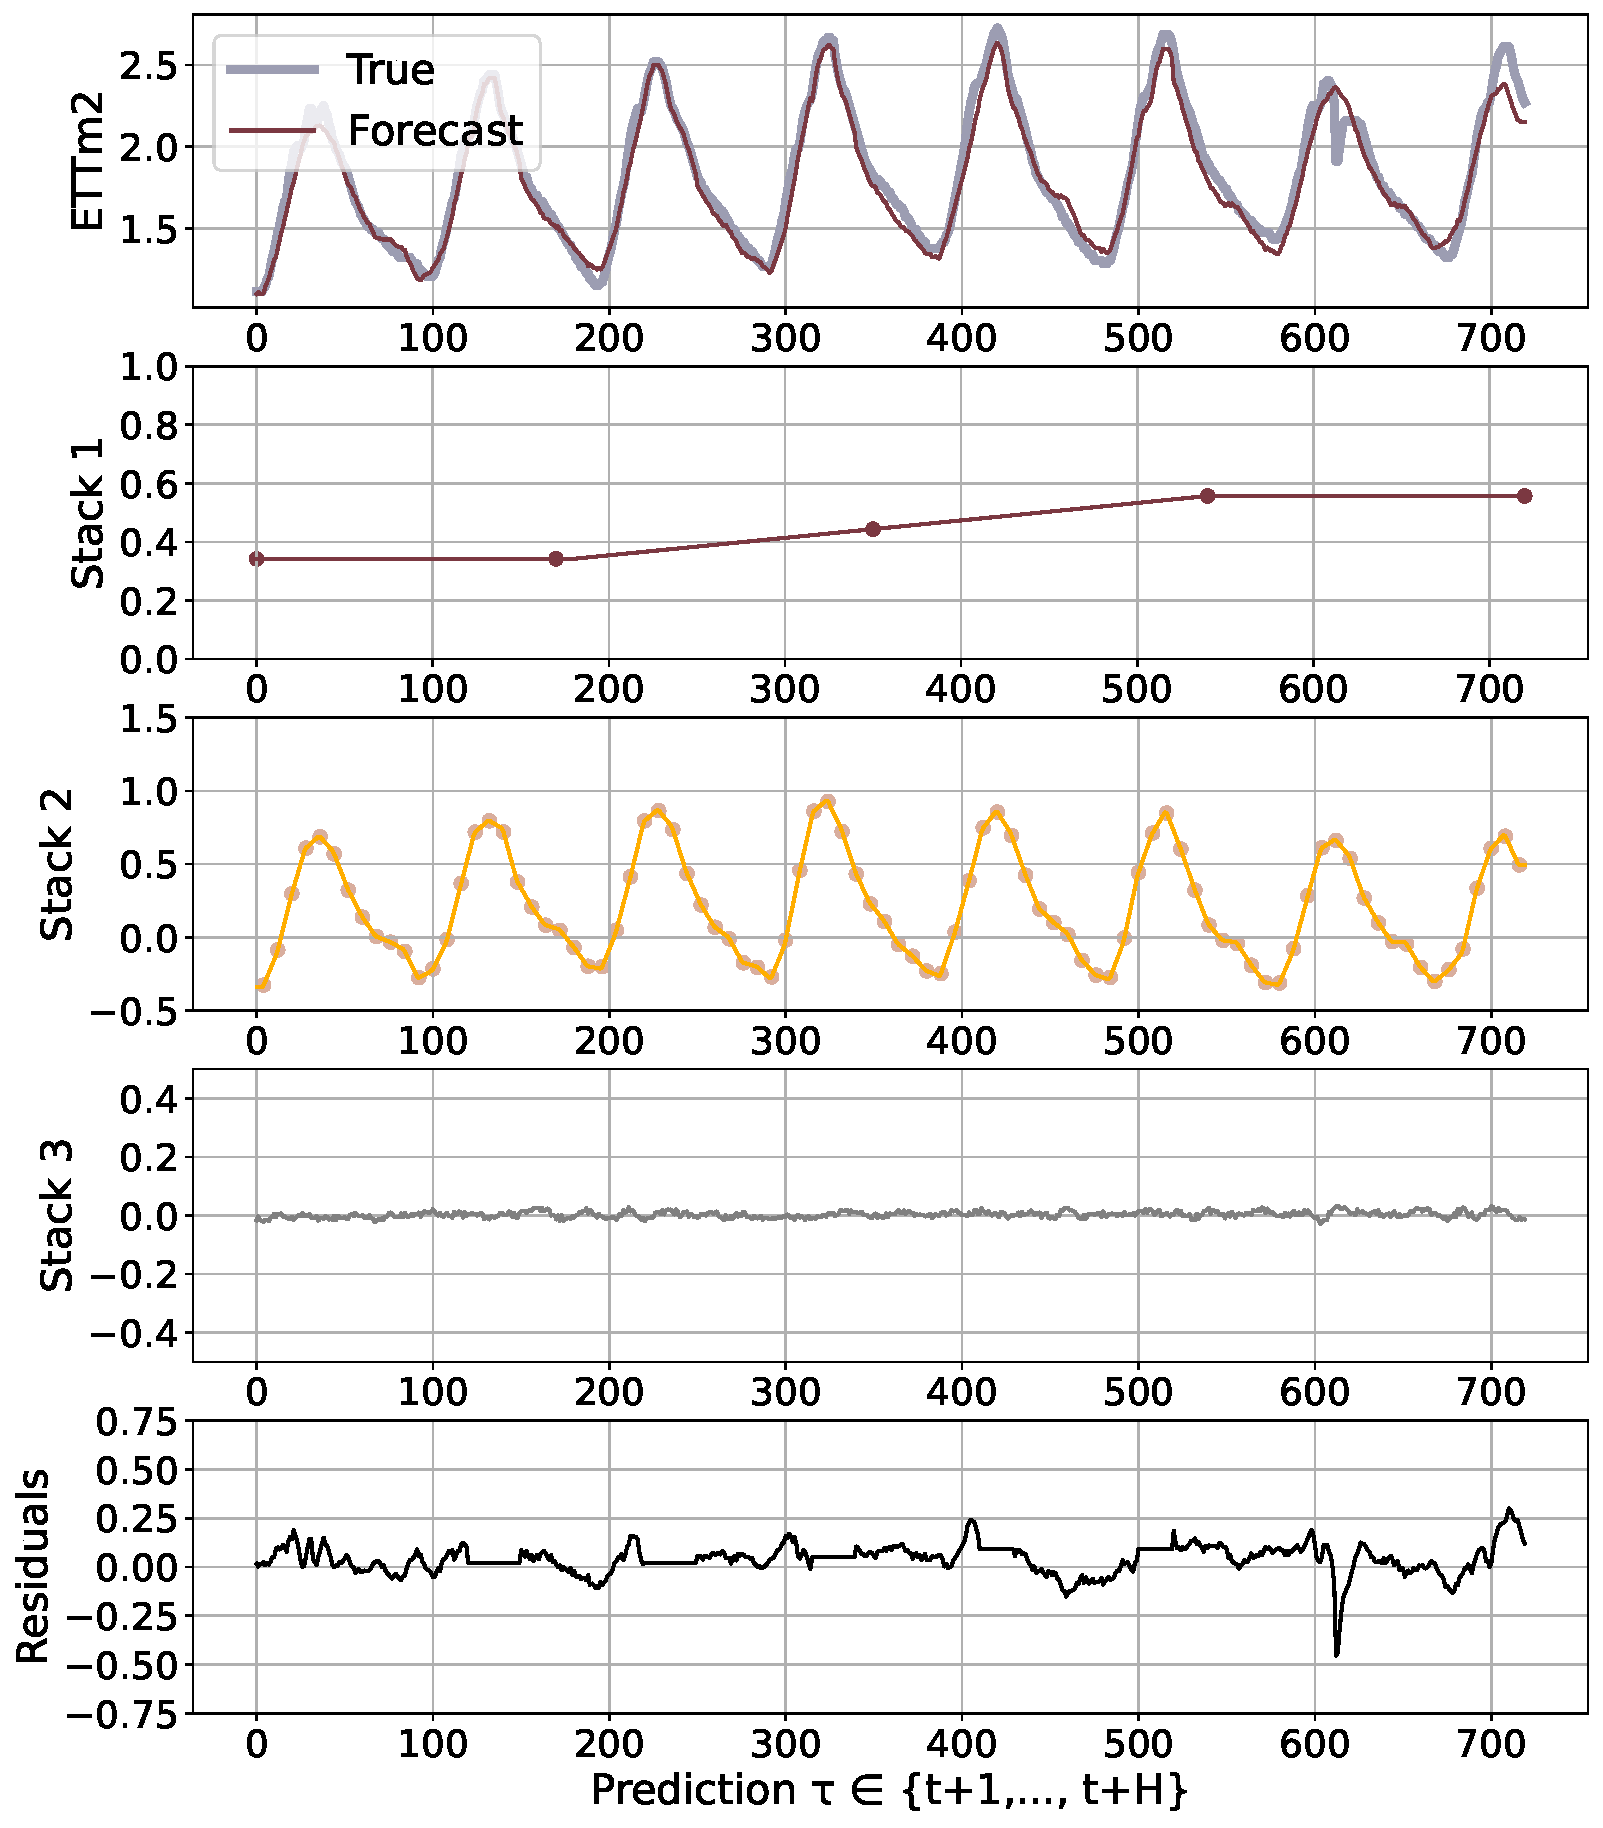
\includegraphics[width=0.48\linewidth]{images/plots-interpetable-decomposition.pdf}}
        ~
        ~
        ~
        ~
\subfigure[Cubic interpolation]{\label{fig:decomposition_cubic}
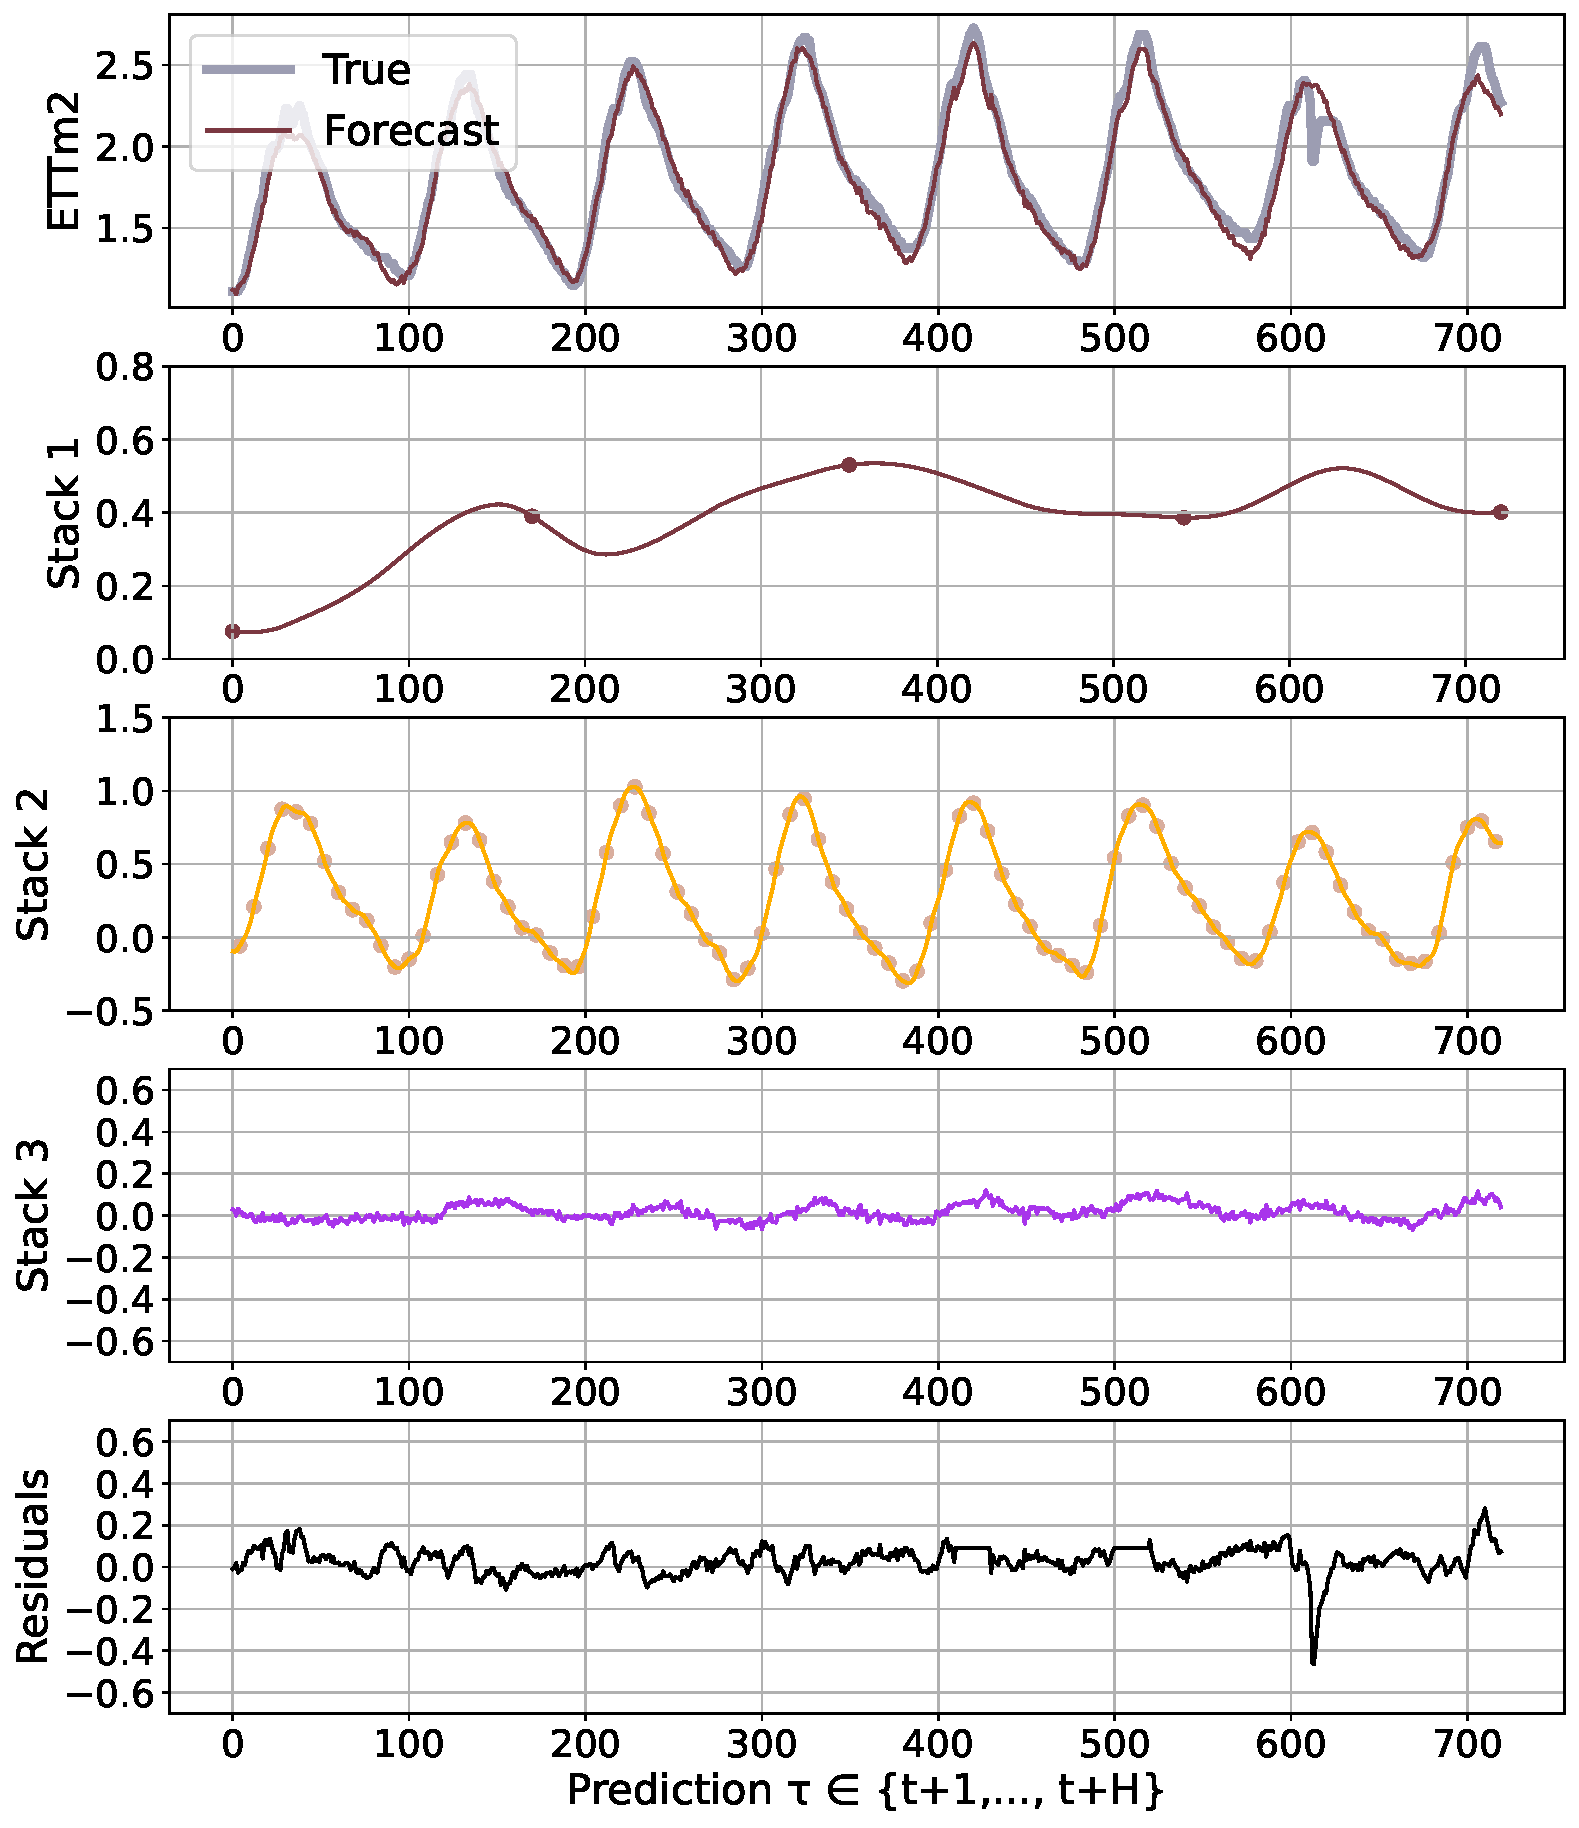
\includegraphics[width=0.48\linewidth]{images/plots-interpetable-decomposition-cubic.pdf}}
\subfigure[No interpolation]{\label{fig:decomposition_generic2}
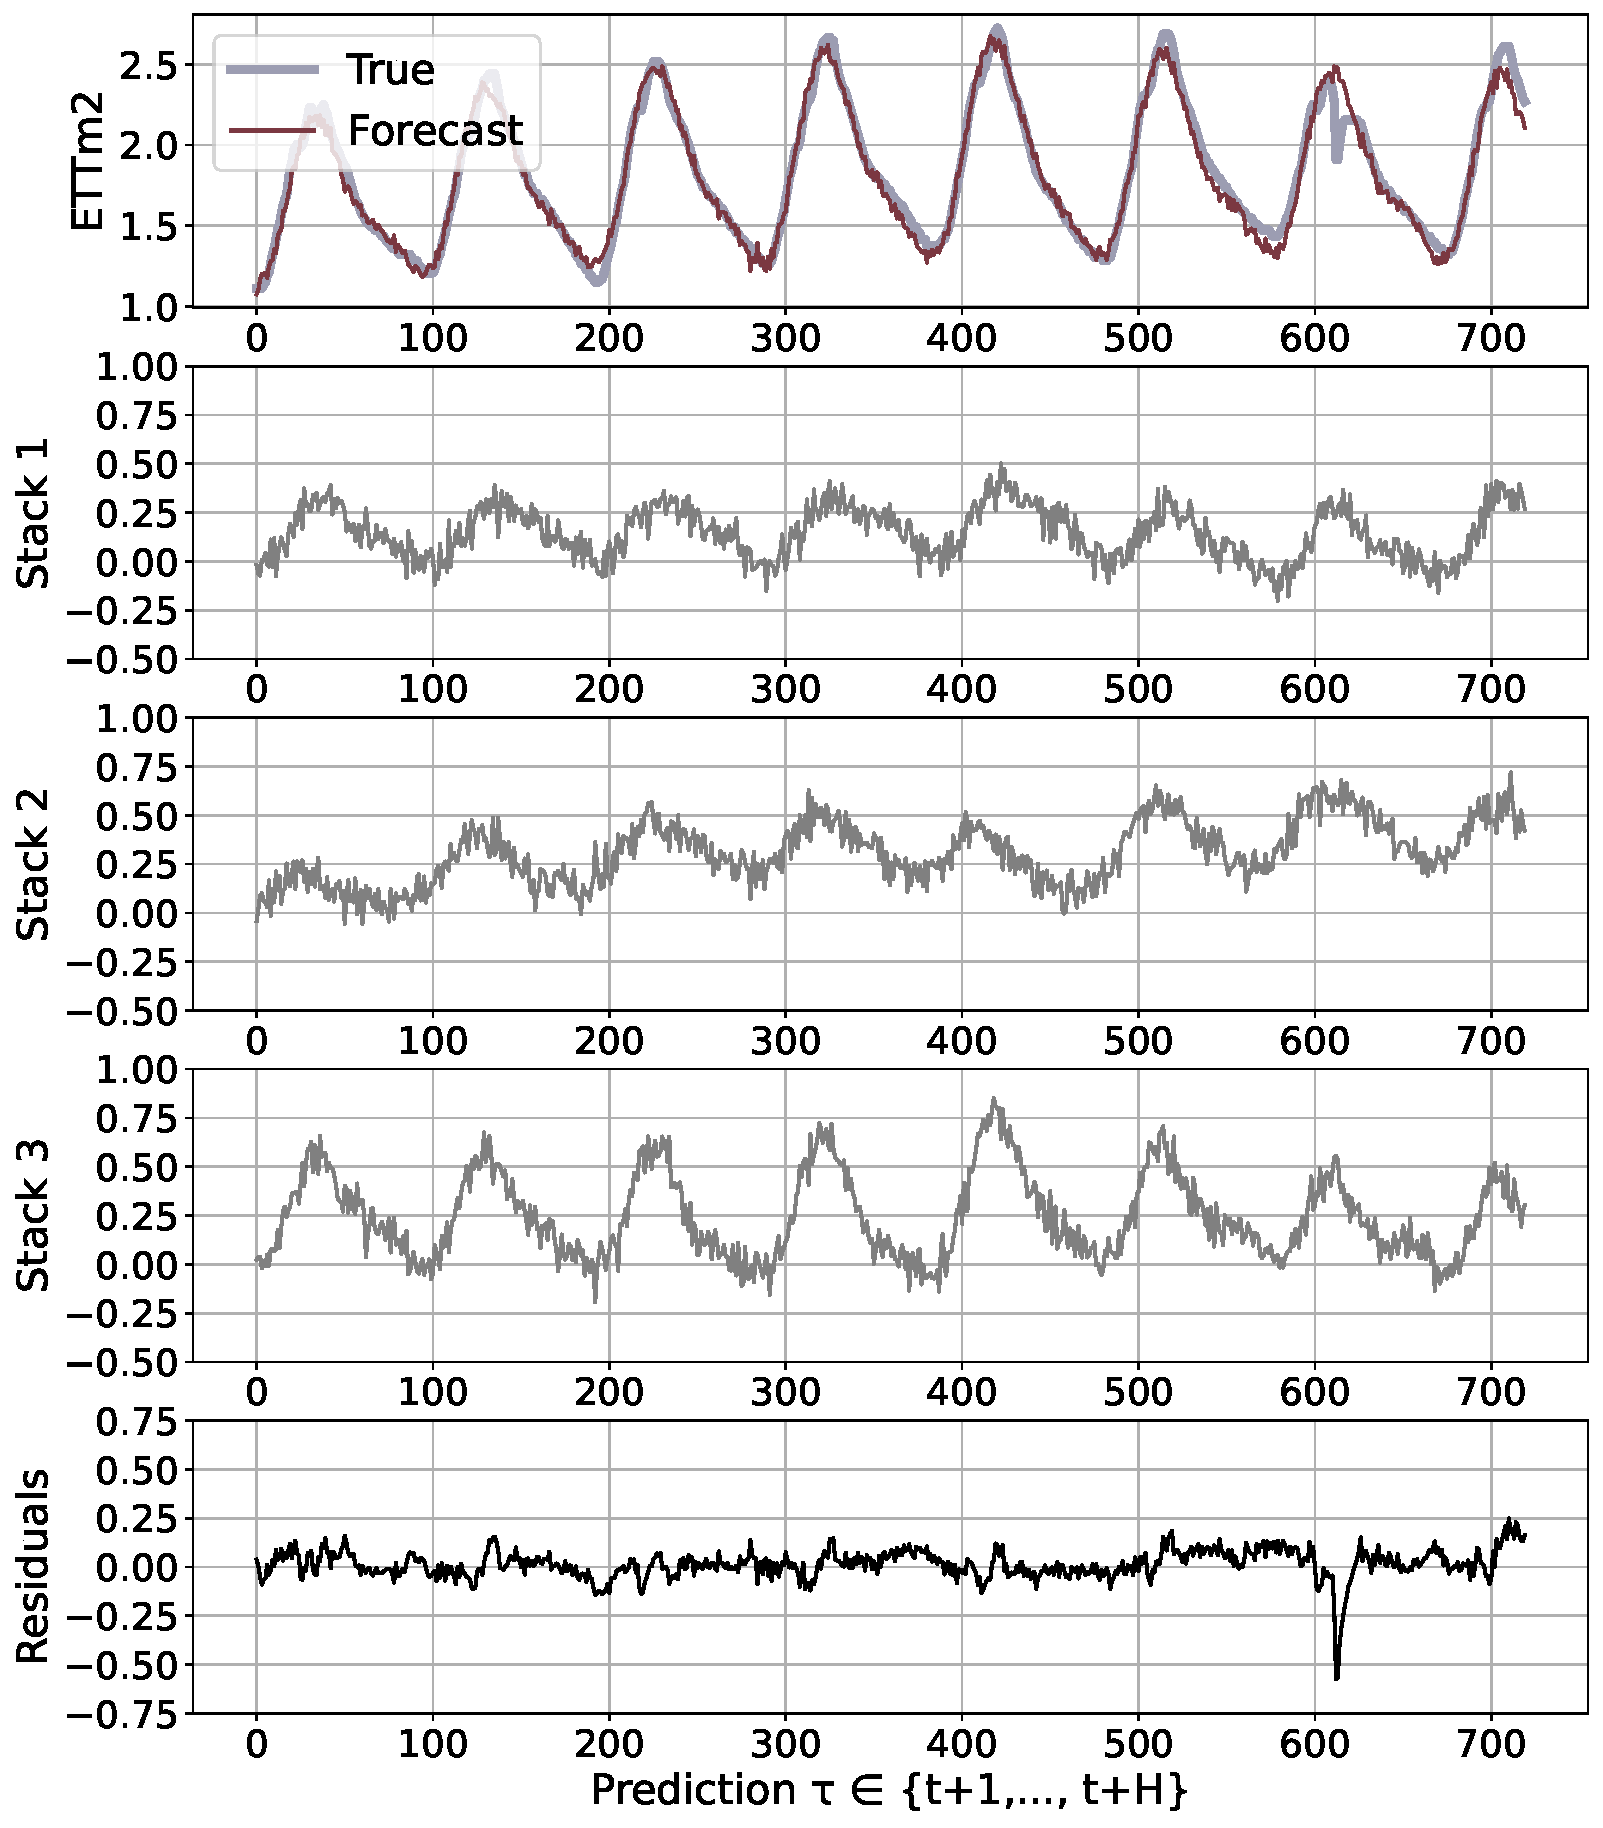
\includegraphics[width=0.48\linewidth]{images/plots-interpetable-decomposition-generic.pdf}}
\vspace{-0.25cm}
\caption{\ETTm2 and 720 ahead forecasts using \ours\ with different interpolation techniques. The top row shows the original signal and the forecast. The second, third and fourth rows show the forecast components across stack, residuals in the last row.} 
\label{fig:decomposition_pooling}
\end{figure*}

The linear interpolation improvements over nearest neighbors are up to 15.8\%, and up to 7.0\% for the cubic interpolation. When comparing between linear and cubic the results are inconclusive as different datasets and horizons slight performance differences. On average across the datasets both the forecasting accuracy and computational performance favors the linear method, with which we conducted the main experiments of this work with this technique.

\begin{table}[ht!] %ht!
%\tiny
\scriptsize
    \begin{center}
    \caption{Empirical evaluation of long multi-horizon multivariate forecasts for \ours\ with different interpolation configurations. All other hyperparameters were kept constant across all datasets. MAE and MSE for predictions averaged over eight seeds, the best result is highlighted in bold (lower is better). Percentage difference relative to n. neighbor in the last panel, average across datasets.}
    \label{table:ablation_interpolation}    
	\begin{tabular}{ll | cccccc} \toprule
    						        &     & \multicolumn{2}{c}{Linear}          & \multicolumn{2}{c}{Cubic}         & \multicolumn{2}{c}{N.Neighbor}  \\
    						        &     & MSE              & MAE              & MSE             & MAE             & MSE            & MAE            \\ \midrule
\parbox[t]{1mm}{\multirow{4}{*}{\rotatebox[origin=c]{90}{\ETTm$_{2}$}}}    						        
									& 96  & 0.185            & 0.265            & \textbf{0.179}  & \textbf{0.256}  & 0.180          & 0.259          \\
									& 192 & 0.244            & 0.308            & \textbf{0.241}  & \textbf{0.303}  & 0.252          & 0.315          \\
									& 336 & \textbf{0.301}   & \textbf{0.347}   & 0.314           &  0.358          & 0.302          & 0.351          \\
									& 720 & \textbf{0.429}   & \textbf{0.438}   & 0.439           &  0.450          & 0.442          & 0.455          \\ \midrule
\parbox[t]{1mm}{\multirow{4}{*}{\rotatebox[origin=c]{90}{\Electricity}}}
									& 96  & 0.152            & 0.257            & \textbf{0.149}  & \textbf{0.252}  & 0.151          & 0.255          \\
									& 192 & \textbf{0.172}   & \textbf{0.275}   & 0.174           &  0.279          & 0.175          & 0.279          \\
									& 336 & 0.197            & 0.304            & \textbf{0.190}  &  \textbf{0.295} & 0.211          & 0.318          \\
									& 720 & \textbf{0.248}   & \textbf{0.347}   & 0.256           &  0.353          & 0.263          & 0.358          \\ \midrule
\parbox[t]{1mm}{\multirow{4}{*}{\rotatebox[origin=c]{90}{\Exchange}}}
									& 96  & \textbf{0.109}   & \textbf{0.232}   & 0.1307          &  0.254          & 0.126          & 0.248          \\
									& 192 & 0.280            & 0.375            & \textbf{0.247}  &  \textbf{0.357} & 0.357          & 0.416          \\
									& 336 & \textbf{0.472}   & \textbf{0.504}   & 0.625           &  0.560          & 0.646          & 0.560          \\
									& 720 & \textbf{1.241}   & \textbf{0.823}   & 1.539           &  0.925          & 1.740          & 0.973          \\ \midrule
\parbox[t]{1mm}{\multirow{4}{*}{\rotatebox[origin=c]{90}{\TrafficL}}}
									& 96  & 0.405            & 0.286            & \textbf{0.402}  & \textbf{0.282}  & 0.405          & 0.359          \\
									& 192 & 0.421            & 0.297            & \textbf{0.417}  & \textbf{0.295}  & 0.419          & 0.201          \\
									& 336 & 0.448            & 0.318            & \textbf{0.446}  & \textbf{0.315}  & 0.445          & 0.253          \\
									& 720 & 0.527            & 0.362            & 0.540           &  0.366          & \textbf{0.525} & \textbf{0.318} \\ \midrule
\parbox[t]{1mm}{\multirow{4}{*}{\rotatebox[origin=c]{90}{\Weather}}}									
									& 96  & 0.164            & 0.199            & 0.162           &  0.203          & \textbf{0.161} & 0.360          \\
									& 192 & 0.224            & 0.255            & 0.225           &  0.257          & \textbf{0.218} & 0.928          \\
									& 336 & \textbf{0.285}   & \textbf{0.311}   & 0.285           &  0.304          & 0.298          & 0.988          \\
									& 720 & \textbf{0.366}   & \textbf{0.359}   & 0.380           &  0.369          & 0.368          & 1.047          \\ \midrule \midrule
\parbox[t]{1mm}{\multirow{4}{*}{\rotatebox[origin=c]{90}{P. Diff.}}}
									& 96  & \textbf{-0.907}  & \textbf{-0.717}  & 0.146           & 1.61            & 0.000          & 0.000          \\
									& 192 & -5.582           & -3.259.          & \textbf{-7.985} & \textbf{-4.332} & 0.000          & 0.000          \\
									& 336 & \textbf{-10.516} & \textbf{-4.199}  & -2.108          & -1.455          & 0.000          & 0.000          \\
									& 720 & \textbf{-15.800} & \textbf{-7.042}  & -5.480          & -1.579          & 0.000          & 0.000          \\ \bottomrule
	\end{tabular}
	\end{center}
\end{table}

% -------------------------------------------------------------------------------------------------------------
% \clearpage
% \newpage
%\vspace{10mm}
\subsubsection{Order of Hierarchical Representations}
\label{appendix:ablation_hierarchy_configurations}
% -------------------------------------------------------------------------------------------------------------

\begin{figure}[!ht]
\centering
\subfigure[\emph{Top-Down}]{\label{fig:hierarchy_descending}
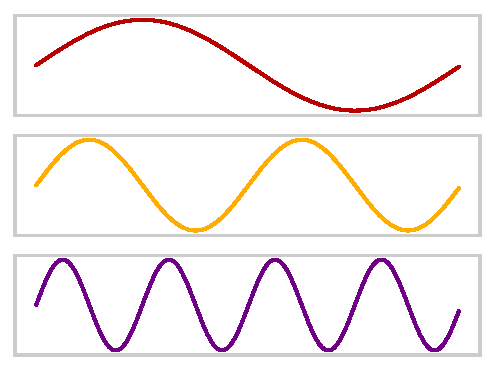
\includegraphics[width=0.28\linewidth]{images/nhits_descending.pdf}}
\subfigure[\emph{Bottom-Up}]{\label{fig:hierarchy_ascending}
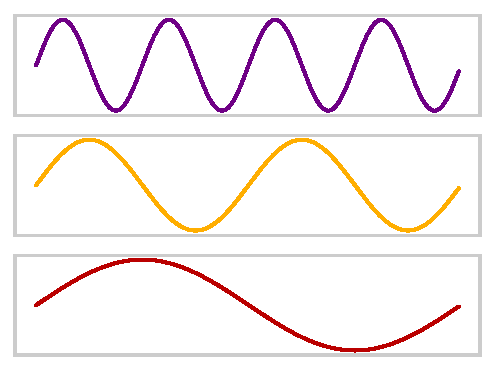
\includegraphics[width=0.28\linewidth]{images/nhits_ascending.pdf}}
\caption{Hierarchical representation configurations.} \label{fig:hierarchies}
\end{figure}

Deep Learning in classic tasks like computer vision and natural language processing is known to learn hierarchical representations from raw data that increase complexity as the information flows through the network. This automatic feature extraction phenomenon is believed to drive to a large degree the algorithms' success \citep{bengio2014hierarchical_representations}. Our approach differs from the conventions in the sense that we use a \emph{Top-Down} hierarchy where we prioritize in the synthesis of the predictions to low frequencies and sequentially complement them with higher frequencies details, as explained in Section~\ref{section3:model}. We achieve this with \ours' \emph{expressiveness ratio} schedules. Our intuition is that the \emph{Top-Down} hierarchy acts as a regularizer and helps the model to focus on the broader factors driving the predictions rather than narrowing its focus at the beginning on the details that compose them. To test these intuitions, we designed an experiment where we inverted the expressiveness ratio schedule into \emph{Bottom-Up} hierarchy predictions and compared the validation performance.

Remarkably, as shown in Table~\ref{table:ablation_hierarchy_order}, the \emph{Top-Down} predictions consistently outperform the \emph{Bottom-Up} counterpart. Relative improvements in MAE are 4.6\%, in MSE of 7.5\%, across horizons and datasets. Our observations match the forecasting community practice that addresses long-horizon predictions by first modeling the long-term seasonal components and then its residuals. %Research on long-horizon forecasting has primarily focused on long-term seasonal component, as it is a common belief that it is the most important.

\begin{table}[ht!] %ht! t
%\tiny
\scriptsize
% \footnotesize
    \begin{center}
    \caption{Empirical evaluation of long multi-horizon multivariate forecasts for \ours\ with different hierarchical orders. All other hyperparameters were kept constant across all datasets. MAE and MSE for predictions averaged over eight seeds, the best result is highlighted in bold (lower is better). Average percentage difference relative to ascending hierarchy in the last panel.}
    \label{table:ablation_hierarchy_order}
	\begin{tabular}{ll | cccccc} \toprule
    						        &     & \multicolumn{2}{c}{Top-Down}       & \multicolumn{2}{c}{Bottom-Up} \\
    						        &     & MSE             & MAE              & MSE            & MAE          \\ \midrule
\parbox[t]{1mm}{\multirow{4}{*}{\rotatebox[origin=c]{90}{\ETTm$_{2}$}}}
									& 96  & \textbf{0.185}  & \textbf{0.265}   & 0.191          & 0.266        \\
									& 192 & \textbf{0.244}  & \textbf{0.308}   & 0.261          & 0.320        \\
									& 336 & \textbf{0.301}  & \textbf{0.347}   & 0.302          & 0.353        \\
									& 720 & \textbf{0.429}  & \textbf{0.438}   & 0.440          & 0.454        \\ \midrule
\parbox[t]{1mm}{\multirow{4}{*}{\rotatebox[origin=c]{90}{\Electricity}}}
									& 96  & \textbf{0.152} & \textbf{0.257}    & 0.164          & 0.270        \\
									& 192 & \textbf{0.172} & \textbf{0.275}    & 0.186          & 0.292        \\
									& 336 & \textbf{0.197} & \textbf{0.304}    & 0.217          & 0.327        \\
									& 720 & \textbf{0.248} & \textbf{0.347}    & 0.273          & 0.369        \\ \midrule
\parbox[t]{1mm}{\multirow{4}{*}{\rotatebox[origin=c]{90}{\Exchange}}}
									& 96  & \textbf{0.109} & \textbf{0.232}    & 0.114          & 0.242        \\
									& 192 & \textbf{0.280} & \textbf{0.375}    & 0.436          & 0.452        \\
									& 336 & \textbf{0.472} & \textbf{0.504}    & 0.654          & 0.574        \\
									& 720 & \textbf{1.241} & \textbf{0.823}    & 1.312          & 0.861        \\ \midrule
\parbox[t]{1mm}{\multirow{4}{*}{\rotatebox[origin=c]{90}{\TrafficL}}}
									& 96  & \textbf{0.405} & \textbf{0.286}    & 0.410          & 0.292        \\
									& 192 & \textbf{0.421} & \textbf{0.297}    & 0.427          & 0.305        \\
									& 336 & \textbf{0.448} & \textbf{0.318}    & 0.456          & 0.323        \\
									& 720 & \textbf{0.527} & \textbf{0.362}    & 0.557          & 0.379        \\ \midrule
\parbox[t]{1mm}{\multirow{4}{*}{\rotatebox[origin=c]{90}{\Weather}}}
									& 96  & 0.164          & \textbf{0.199}    & \textbf{0.163} & 0.200           \\
									& 192 & 0.224          & 0.255             & \textbf{0.219} & \textbf{0.252}  \\
									& 336 & \textbf{0.285} & \textbf{0.311}    & 0.288          & 0.311           \\
									& 720 & 0.366          & 0.359             & \textbf{0.365} & \textbf{0.355}  \\ \midrule \midrule
\parbox[t]{1mm}{\multirow{4}{*}{\rotatebox[origin=c]{90}{P. Diff.}}}
									& 96  & \textbf{-2.523}  & \textbf{-2.497} & 0.000          & 0.000        \\
									& 192 & \textbf{-12.296} & \textbf{-6.793} & 0.000          & 0.000        \\
									& 336 & \textbf{-11.176} & \textbf{-5.507} & 0.000          & 0.000        \\
									& 720 & \textbf{-4.638}  & \textbf{-3.699} & 0.000          & 0.000        \\ \bottomrule
	\end{tabular}
	\end{center}
\end{table}
